\section {The NFActor System}

\begin{figure}[!t]
  \centering
  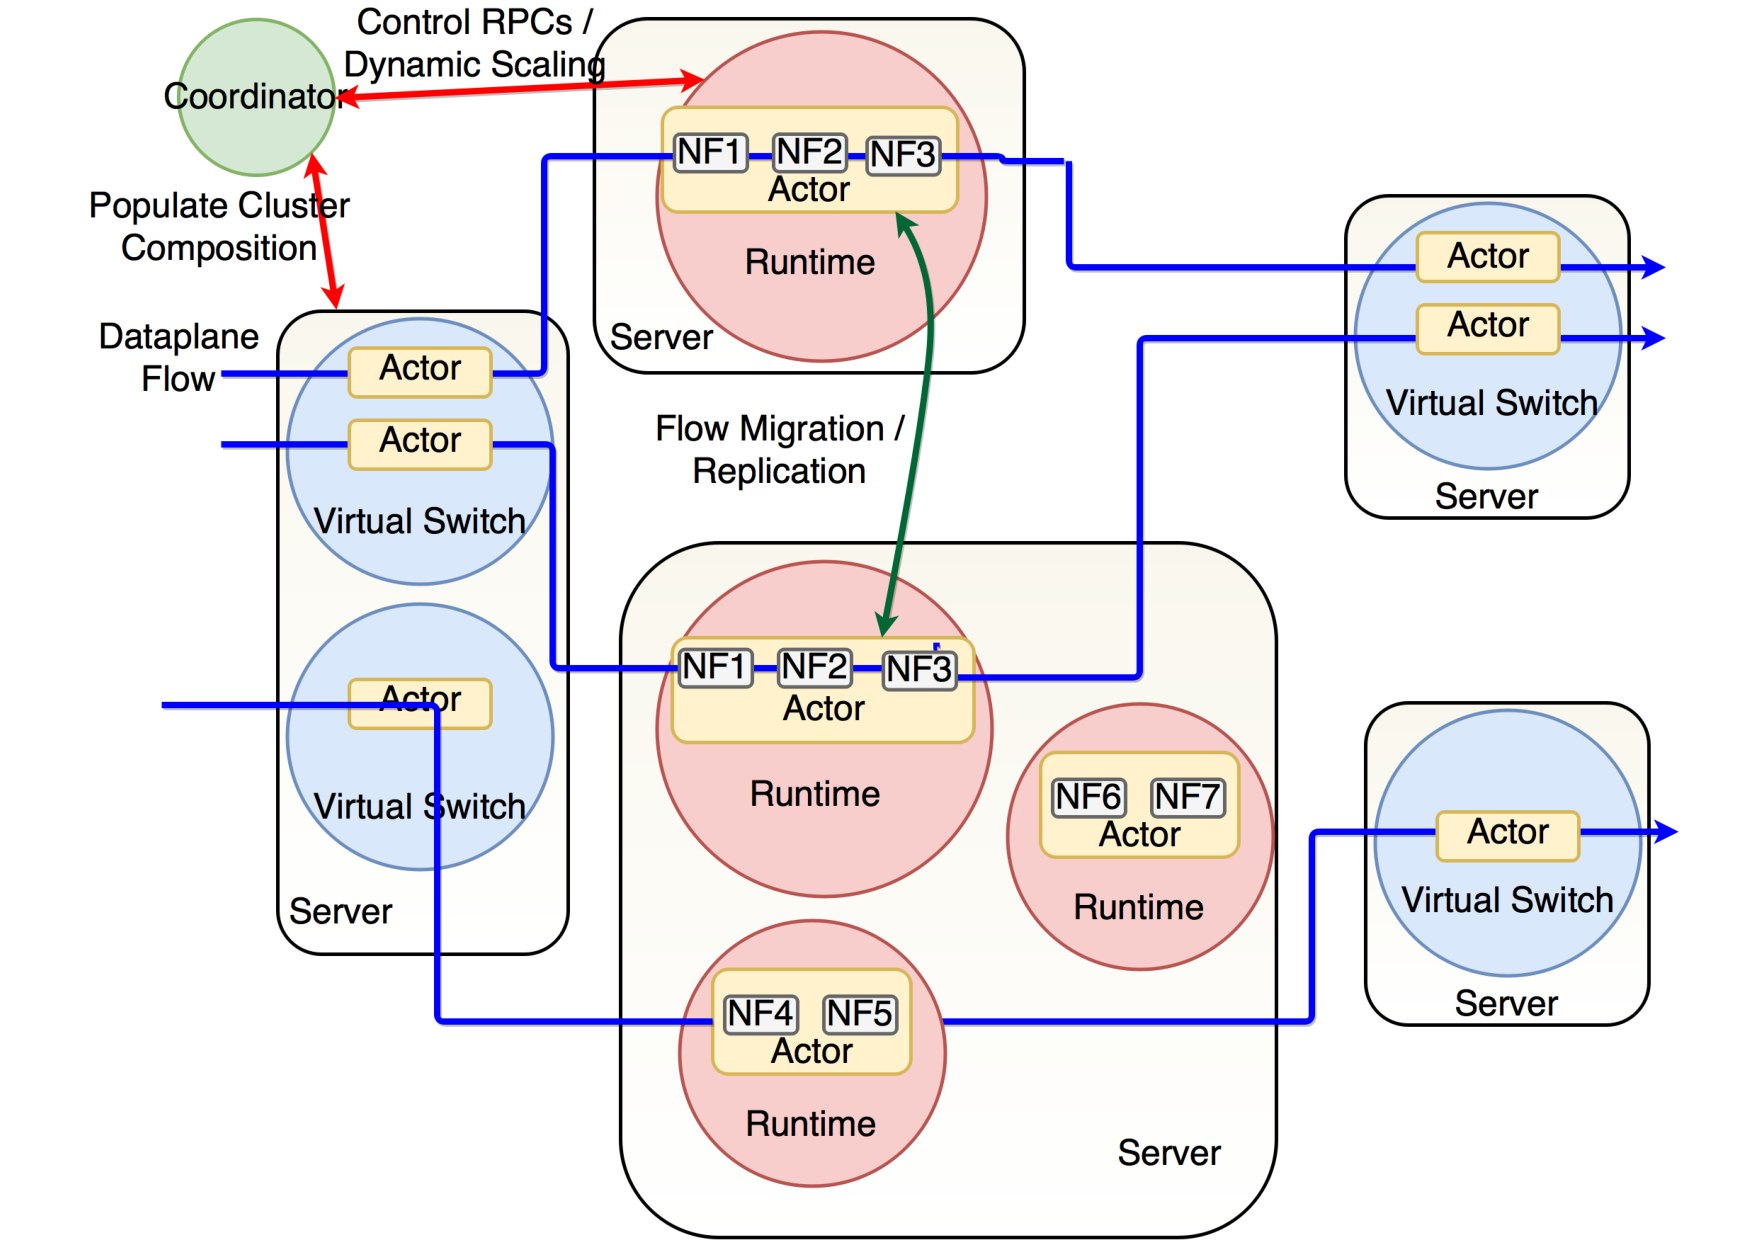
\includegraphics[width=\columnwidth]{figure/new-nfactor-cluster.pdf}
  \caption{An overview of \nfactor.}
  \label{fig:runtime}
\end{figure}

We present the design and key modules of \nfactor~in this section.

\subsection{Overview}
\label{sec:overview}

\nfactor~includes three key modules: (i) runtime systems that enable flow processing using actors; (ii) virtual switches for distributing and balancing flows to runtime systems; and (iii) a light-weight coordinator for basic system management. % (\eg, runtime load monitoring and scaling, participate in the initiation phase of flow migration and replication).
 An illustration of the architecture of \nfactor~is given in Fig.~\ref{fig:runtime}.

A runtime system, referred to as \textit{runtime} for short, is the execution environment of NFs and service chains. A runtime is running on a container, for quick launching and rebooting in cases of scaling up and failure recovery. There can be multiple runtimes (containers) running on the same physical server. In \nfactor, the virtual switches are running in the same environments (containers) as those runtimes and run actors for flow distribution, \ie, a virtual switch can be regarded as a special runtime that runs a load balancer function. Runtimes and virtual switches are inter-connected through a L2 network.

%When a dataplan flow arrives in the system, it is first sent to a virtual switch.
The virtual switch is configured with an entry IP address and the coordinator sets up corresponding flow rules to direct the dataplane flow to the virtual switch,%\chuan{clarify how a flow gets to be sent to a virtual switch, by knowing its IP address or being sent by the coordinator?},
 which dispatches it to a runtime hosting the NF service chain that the flow is to traverse (Sec.~\ref{sec:virtualswitch}). When a runtime receives a new flow, it creates a new flow actor to process the flow. Our runtime design follows the one-actor-one flow principle (Sec.~\ref{sec:runtime}): the flow actor loads all the required NFs of the service chain, and passes the received packets of the flow to these NFs in sequence. %of the service chain.
 Once a packet has been processed by all NFs in the service chain, the runtime sends the packet to another virtual switch,
%(which can be the same or a different virtual switch where the flow comes into the system),
where the packet is forwarded to its destination (the packet will be forwarded out by the replica flow actor when the failure resilience mechanism is in place Sec.~\ref{sec:resilience}).



%The key feature that differentiates NFActor framework from the existing works like \cite{gember2015opennf} and \cite{rajagopalan2013split} is that, resilience operations, \ie~flow migration and replication, is fully decentralized. Figure \ref{fig:runtime} demonstrates a flow migration process that migrates actor 2 on runtime 1 to runtime 2. \ac{The migration starts by actor 2 sending the first request to runtime 2. Runtime 2 launches actor 4, which is used as the migration target actor for accepting the flow packets and flow states of actor 2, before responding to actor 2. Actor 2 then sends the second request to the virtual switch, asking it to modify the output route to runtime 2. Finally, actor 2 sends its flow states in the third request to actor 4, completing the whole migration process. The details of our distributed flow migration is further illustrated in \ref{}.} \cui{The third paragraph on describing flow migration is not clear. Should make it more clear, or make it the "Section 3.1 Example" section, or cut this paragraph.}

The coordinator in \nfactor~is responsible for basic cluster management (Sec.~\ref{sec:controller}), \eg, updating latest cluster composition to the virtual switches and runtimes, monitoring workload of runtimes, control dynamic scaling. % and participate in the initiation phase of flow migration and replication.
As compared to SDN controllers used in the existing NFV management systems \cite{gember2015opennf, rajagopalan2013split}%\chuan{add citations}
, the coordinator is much lightweight, without involving in the entire flow migration and replication process.%xxx \chuan{complete}.
 Instead, flow migration and replication are handled in fully distributed fashion among flow actors, and only exploit the coordinator in the initialization phase.
%our main observration is that actor privdes the unique feature to implement a high throughput system due to its light-weight execution state and and

%%%light-weight, decentralized migration of network flow states

%Our main observation is that actor provides the unique benefits for light-weight, decentralized migration of network flow states.

The design of \nfactor~targets the following goals. %\chuan{complete the following. each bullet 2-3 sentences}

{\bf 1. Transparent Resilience.} Flow actor should be able to transparently perform resilience operations, including flow migration and replication, regardless of the service chain that is configured for it. %The NF modules implemented using the module API (Sec.~\ref{sec:module-api}) should be transparently

{\bf 2. High Scalability.} The runtime should have good horizontal scalability so that~\nfactor~could easily scale-up by launching additional runtimes.

{\bf 3. Low Overhead.} High speed packet processing must be achieved by~\nfactor~framework to suit the requirement of modern NFV system.
